\documentclass[a4paper,twoside,onecolumn,openany,article]{memoir}
\usepackage{xeCJK}
\usepackage{url}
\usepackage{tikz}
\usepackage{hyperref}
\usepackage{amsmath}
\usepackage{amssymb}
\usepackage{amsthm}
\usepackage{algpseudocode}
\usepackage{algorithm}
\defaultfontfeatures{Ligatures=TeX}

\setCJKmainfont[BoldFont=IPAGothic]{IPAMincho}
\setCJKsansfont{IPAGothic}
\setCJKmonofont{IPAGothic}

\theoremstyle{remark}
\newtheorem{remark}{\bf 余談}


%\setmainfont{}
\setsansfont{URW Gothic}
\setmonofont{Inconsolata}

\usepackage{listings}



\settrimmedsize{\stockheight}{\stockwidth}{*}

%\setlrmarginsandblock{1.5in}{1in}{*}
\setlrmarginsandblock{1.5in}{1.5in}{*}
\setulmarginsandblock{1.3in}{1.5in}{*}
\setheadfoot{20mm}{15mm}

%\newlength{\linespace}
%\setlength{\linespace}{\baselineskip}
%\setlength{\headheight}{\onelineskip}
%\setlength{\headsep}{\linespace}
%\addtolength{\headsep}{-\topskip}

%\setlength{\footskip}{\onelineskip}
%\setlength{\footnotesep}{\onelineskip}

\checkandfixthelayout

\counterwithout{section}{chapter}
\setsecnumdepth{subsubsection}

\title{計算機科学第一}
\date{12月15日}

\begin{document}
\maketitle

\noindent
今週の目標
\begin{itemize}
\item クラスに慣れる。乱数を使えるようになる。
\end{itemize}

\noindent
今日の課題(提出締切は年明けの最初の演習の時間が始まるまで)
\begin{enumerate}
\item 
グラフのクラスを作り、ランダムグラフを生成するプログラムを書く。
\item
グラフのクラスに最大連結成分のサイズを返すメソッドを実装し、最大連結成分のサイズの平均値を数値実験で評価する。
\end{enumerate}

\noindent
今日のワークフロー
\begin{enumerate}
\item 今まで通り
\end{enumerate}

\section{グラフ}
グラフとは頂点の集合$V$と枝の集合$E\subseteq V\times V$のペアのことです。
例えば$(V=\{1,2,3,4, 5\}, E=\{(1,2),(2,3),(3,4),(4,1)\})$は頂点数5、枝数4のあるグラフを表しています。
グラフは図で表現することもできます。上記の例の場合、

\begin{center}
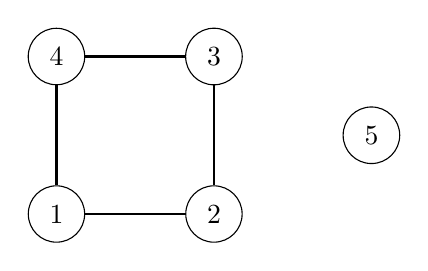
\begin{tikzpicture}
\node[draw, circle, inner sep=0.15cm] (1) at (0,0) {1};
\node[draw, circle, inner sep=0.15cm] (2) at (2,0) {2};
\node[draw, circle, inner sep=0.15cm] (3) at (2,2) {3};
\node[draw, circle, inner sep=0.15cm] (4) at (0,2) {4};
\node[draw, circle, inner sep=0.15cm] (5) at (4,1) {5};
\draw (1.east) to (2.west) [thick];
\draw (2.north) to (3.south) [thick];
\draw (4.east) to (3.west) [thick];
\draw (1.north) to (4.south) [thick];
\end{tikzpicture}
\end{center}
という図がグラフを表現しています。
枝を表すペアの中の順序の違いは区別しないとします(枝$(1,2)$と$(2,1)$は同じ意味)。
互いに枝を通って辿り着ける頂点の部分集合で極大であるものを連結成分と呼びます。上記の例の場合$\{1,2,3,4\}$と$\{5\}$が連結成分です。
 
\section{疑似乱数}
確率的に値が決まる数のことを計算の文脈では乱数と呼びます。
現実のコンピュータでは基本的には確定的な値のみを扱うので本当の意味での乱数は現れません。
しかししばしば周期が長い数列を確定的な計算で生成し乱数列の代わりとして扱います。
このように確定的な計算によって作られた周期の長い数列のことを疑似乱数列と呼びます。
Scala では \texttt{scala.util.Random} を使って以下のように疑似乱数を得ることができます。
%\texttt{import scala.util.Random} としてから
\begin{verbatim}
import scala.util.Random
val rng = new Random
rng.nextDouble
rng.nextInt
rng.nextInt(10)
\end{verbatim}
ここで \texttt{rng.nextDouble} は 0より大きく1より小さい範囲の Double型の値を一様な確率で(擬似的にですが)返します。
また \texttt{rng.nextInt} は Int 型の値の中で一様な確率で値を返します。
また \texttt{rng.nextInt(n)} は 0以上 \texttt{n}未満の Int 型の値を一様な確率で値を返します。
ここで \texttt{rng} は内部に状態を持っており \texttt{rng.nextDouble} を複数回呼んだときには毎回違った値が得られます。

このように疑似乱数を用いることでランダムな計算をすることができますが、参照透過性(関数の出力は入力のみによって決まる)のために
ランダムな計算をする関数には引数として \texttt{Random} 型を渡してください。
例えば Double型の値 \texttt{x} を受け取り疑似乱数を足して返す関数は
\begin{verbatim}
def addRandom(x: Double, rng: Random) = x + rng.nextDouble
\end{verbatim}
と書いてください。
また、疑似乱数はテストをする上でも有用です。

\section{課題について}
\subsection{概要}
Graph クラスを作り、疑似乱数を使ってランダムグラフを生成するプログラムを作ってください。
ここでパラメータ $n$ と $p$ を持つランダムグラフは$n$個の頂点を持ち $\binom{n}{2}$個の頂点のペアをそれぞれ独立に確率$p$で枝として持つものとします。
このランダムグラフの最大連結成分の平均サイズを実験的に評価してください。
確率 $p$ を $c/n$ とした場合のランダムグラフの最大連結成分の平均サイズを$s(n,c)$ とした場合に $s(n,c)$ を $c=0.1,\, 0.2,\dotsc, 1.9,\, 2.0$, $n=10,\, 50,\, 100,\, 500$
の場合に疑似乱数を用いた数値実験で評価してください。
相対的な最大連結成分の平均サイズ$s(n,c)/n$は $n\to\infty$極限である関数に収束します。その値が\texttt{giant.txt} に書かれているので数値実験結果と比較できるように gnuplotで図を作ってください。

\subsection{Graph クラス}
Graphクラスを以下のように定義します。
\begin{verbatim}
class Graph(n: Int, e: List[(Int, Int)]) {
  val size: Int = n
  val edges: List[(Int, Int)] = e
}
\end{verbatim}
ここで \texttt{size} は頂点数 、\texttt{edges}は枝の集合を表わすものとします。
頂点の集合は0から$\mathtt{size}-1$までの整数の集合とします。
頂点を表わす整数を受け取り、その頂点と接続している頂点のリストを返す関数 \texttt{neighbors} を実装してください。
また最大連結成分のサイズを返す関数 \texttt{maximumComponent}を実装してください(幅優先探索もしくは深さ優先探索で計算するのがよいと思います)。

次に \texttt{RandomGraph} オブジェクトの \texttt{genRandomGraph} メソッド(ランダムグラフを生成するメソッド)を実装してください。
これらが完成したら疑似乱数を用いた数値実験でランダムグラフの最大連結成分の平均サイズを評価してください。
そのためには \texttt{main}関数の一行目の\texttt{var n = 10} の部分を編集するだけでよいです。
この 10 の部分を実験したい頂点数に書き換えて実行すると計算結果がファイルに書き込まれます。
私が書いたプログラムだと $n=500$ の場合に演習室で約30分の実行時間がかかりました。

\subsection{gnuplot}
得られた計算結果を図にプロットしてみましょう。
ターミナルからコマンド gnuplot を実行して
\begin{verbatim}
gnuplot> plot [0:2] "10_100000.txt" w l, "50_20000.txt" w l, "100_10000.txt" w l,
 "500_2000.txt" w l, "giant.txt" w l
\end{verbatim}
とすれば図がプロットされます。
この図をpdfファイルに出力するには
\begin{verbatim}
gnuplot> set term pdf
gnuplot> set output "rg_maximum_component.pdf"
gnuplot> set xlabel "average degree"
gnuplot> set ylabel "relative size of the maximum component"
gnuplot> plot [0:2] "10_100000.txt" w l, "50_20000.txt" w l, "100_10000.txt" w l,
 "500_2000.txt" w l, "giant.txt" w l
\end{verbatim}
とすればよいです。

\subsection{提出物}
数値計算で得られたファイル
\texttt{10\_100000.txt, 50\_20000.txt, 100\_10000.txt, 500\_2000.txt}
と gnuplot で出力した図 \texttt{rg\_maximum\_component.pdf}
をレポジトリに追加してください。テストは\texttt{neighbors} についてやってください。
提出方法は今までと同じです。

もっと大きなサイズ $n= 1000$ や $n=10000$ について計算してレポジトリに追加してもよいです。


\end{document}
